\documentclass[journal]{IEEEtran}

\ifCLASSINFOpdf
 \usepackage[pdftex]{graphicx}
  % declare the path(s) where your graphic files are
  % \graphicspath{{../pdf/}{../jpeg/}}
  % and their extensions so you won't have to specify these with
  % every instance of \includegraphics
  % \DeclareGraphicsExtensions{.pdf,.jpeg,.png}
\else
  % or other class option (dvipsone, dvipdf, if not using dvips). graphicx
  % will default to the driver specified in the system graphics.cfg if no
  % driver is specified.
  % \usepackage[dvips]{graphicx}
  % declare the path(s) where your graphic files are
  % \graphicspath{{../eps/}}
  % and their extensions so you won't have to specify these with
  % every instance of \includegraphics
  % \DeclareGraphicsExtensions{.eps}
\fi



\usepackage{amsmath}
%\usepackage{amsaddr}		
%\usepackage{amsthm}		
%\usepackage{amsaddr}		
\usepackage{amsfonts}		



%DEFS. RODNEY%%%%%%%%%%%%%%%%%%%%%%%%%%%%%%%%%%%%%
\def\bSig\mathbf{\Sigma}
\newcommand{\VS}{V\&S}
\usepackage{url}
\usepackage{soul} % allows to pass a line in words
\newcommand{\Z}{\mathbb{Z}} % Set of integers
\newcommand{\re}{\mathbb{R}} % Set of real numbers
\newcommand{\sgn}{\mathrm{sign}} % Signal operador
\newcommand{\ci}{\mathrm{i}}
\def\sT{\mbox{\tiny$T$}}
\def\E{\mbox{{\rm E\,}}}
\def\cov{\mbox{{\rm cov\,}}}
\def\corr{\mbox{{\rm corr\,}}}
\def\var{\mbox{{\rm var\,}}}
\newcommand{\vgamma}{\pmb{\gamma}}
\newcommand{\vrho}{\pmb{\rho}}
\newcommand{\vbeta}{\pmb{\beta}}
\newcommand{\vxi}{\pmb{\xi}}
\newcommand{\vepsilon}{\pmb{\epsilon}}
\def\shalf{\mbox{{\tiny$\frac{1}{2}$}}}
\def\half{\mbox{{\small$\frac{1}{2}$}}}
%\newtheorem{theorem}{Theorem}{\bf}{\rm}  
\newtheorem{lemma}{Lemma}

\newcommand{\vA}{{\textbf A}}
\newcommand{\vD}{{\textbf D}}
\newcommand{\vd}{{\textbf d}}
\newcommand{\vW}{{\textbf W}}
\newcommand{\vR}{{\textbf R}}
\newcommand{\vS}{{\textbf S}}
\newcommand{\vU}{{\textbf U}}
\newcommand{\vI}{{\textbf I}}
\newcommand{\vX}{{\textbf X}}
\newcommand{\vf}{{\textbf f}}
\newcommand{\vu}{{\textbf u}}
\newcommand{\vT}{{\textbf T}}
\newcommand{\vt}{{\textbf t}}


\usepackage{hyperref}

%DEFS. ROGERIO%%%%%%%%%%%%%%%%%%%%%%%%%%%%%%%%%%%%
%\usepackage{graphicx}

\usepackage{subfigure}
\usepackage{multirow}
\usepackage{color,colortbl}
\usepackage{enumerate}
\usepackage{amsmath,amssymb}
\usepackage{booktabs}
\usepackage{rotating}
\usepackage{cite}
\usepackage{balance}

\usepackage{bm,bbm}
\usepackage{datetime2}
\usepackage[binary-units]{siunitx}

\usepackage{mathrsfs}

\usepackage{placeins}

\usepackage[abs]{overpic}
\usepackage{pict2e}
%\usepackage{float}
\usepackage{microtype}
\usepackage{pdfpages}

\makeatletter
\newcommand{\thickhline}{\noalign {\ifnum 0=`}\fi \hrule height 1pt \futurelet \reserved@a \@xhline}
\newcolumntype{"}{@{\hskip\tabcolsep\vrule width 1pt\hskip\tabcolsep}}
\makeatother
%%%%%%%%%%%%%%%%%%%%%%%%%%%%%%%%%%%%%%%%%%%%%%%%%%





% correct bad hyphenation here
%\hyphenation{op-tical net-works semi-conduc-tor}


\begin{document}
\title{Wavelet Spatio-Temporal Change Detection on multi-temporal SAR images}

\author{Rodney~V.~Fonseca, Rog\'{e}rio~G.~Negri,
        Alu\'{i}sio~Pinheiro,
        and~Abdourrahmane~Atto,~\IEEEmembership{Senior~Member,~IEEE}% <-this % stops a space
\thanks{This work was supported by FAPESP (Grants 2016/24469-6, 2018/04654-9 and 2021/01305-6) and CNPq (Grants 309230/2017-9 and 310991/2020-0).}
\thanks{R.~Fonseca and A.~Pinheiro are with the Department of Statistics, University of Campinas, Campinas 13083-859, Brazil (e-mails: ra192588@dac.unicamp.br; pinheiro@ime.unicamp.br).}
\thanks{A.~Atto is with the LISTIC - Polytech Annecy-Chamb\'{e}ry, Universit\'{e} de Savoie, 74944 Annecy le Vieux Cedex, France (e-mail: Abdourrahmane.Atto@univ-savoie.fr).}
\thanks{R.~G.~Negri are with the Department of Environmental Engineering, São Paulo State University, São José dos Campos, Brazil (e-mail: rogerio.negri@unesp.br).}
}
% <-this % stops a space
%\thanks{Manuscript received April 19, 2005; revised August 26, 2015.}}


% The paper headers
\markboth{Journal of \LaTeX\ Class Files,~Vol.~X, No.~X, Month~20XX}%
{Shell \MakeLowercase{\textit{et al.}}: Bare Demo of IEEEtran.cls for IEEE Journals}


% make the title area
\maketitle

% As a general rule, do not put math, special symbols or citations
% in the abstract or keywords.
\begin{abstract}
We introduce WECS (Wavelet Energies Correlation Screening), an unsupervised sparse procedure to detect spatio-temporal change points on multi-temporal SAR images or even on sequences of very high resolution images. The procedure is based on multiscale approximation for the multi-temporal images, wavelet energy apportionment, and ultra-high dimensional correlation screening for the wavelet coefficients. We present two complimentary multiscale measures in order to detect sudden and/or cumulative changes, as well as for the case of stationary or non-stationary multi-temporal images. We show WECS performance on synthetic multi-temporal image data. We also apply the proposed method to a time series of 85 satellite images in the border region of Brazil and the French Guiana. The images were captured from November 08, 2015 to December 09 2017. \textcolor{magenta}{(lapidaremos ao fim)}
\end{abstract}

% Note that keywords are not normally used for peerreview papers.
\begin{IEEEkeywords}
Change detection, multi-temporal images, satellite images, wavelets.
\end{IEEEkeywords}


% For peer review papers, you can put extra information on the cover
% page as needed:
% \ifCLASSOPTIONpeerreview
% \begin{center} \bfseries EDICS Category: 3-BBND \end{center}
% \fi
%
% For peerreview papers, this IEEEtran command inserts a page break and
% creates the second title. It will be ignored for other modes.
\IEEEpeerreviewmaketitle



\section{Introduction}

%%%RGN: Iniciar com uma visão geral do problema (detecćão de mudanća em dados multitemporais). O que é (a ideia)? Porque é importante? Mencionar abordagens supervisionada e não supervisionadaA inclusão de um/dois parágrafos seria suficiente. laplace

\textcolor{red}{\IEEEPARstart{C}{hange} detection... (completar)...}



A review for change detection in multi-temporal remote sensing is given by \cite{ban2016change}. 
Different proposals for this purpose may be found  in the literature. They vary in their motivations as well as in their applicability.  Change detection in multi-temporal hyperspectral images is discussed in \cite{bovolo2015time},  \cite{liu2019review}, and \cite{matsunaga2017current}.  \cite{jia2018novel} pursue change detection techniques via non-local means and principal component analysis. Compressed projection and image fusion are employed by \cite{hou2014unsupervised}. Deep learning by slow feature analysis for change detection is the subject of \cite{du2019unsupervised}. \cite{chen2020change} proposes a change detection method driven by adaptive parameter estimation.


%%%RGN: Eu acho muito interessante que esta pesquisa esteja destinada à dados SAR (lida bem com dados ruidosos, imagens de uma única banda/polarizaćão e contempla uma aplicaćão real com dados Sentinel), no entanto, sinto falta de uma justificativa que relacione o método à dados SAR.


%%%RGN: Podemos omitir o "via polarimetric SAR (POLSAR)"?
Besides different methodological paradigms, several areas of application receive special attention.  For instance, urban change detection applications via polarimetric SAR (POLSAR) images are discussed in \cite{ansari2020urban}. \cite{song2018multi} discusses land cover change detection in mountainous terrain via multi-temporal and multi-sensor remote sensing images. \cite{ru2021multi} studies multi-temporal scene classification and scene change detection. Deforestation change detection is discussed by \cite{barreto2016deforestation}. 



%%%RGN: o "wavelet methods" aqui não está claro se é destinado à detecćão de mudanćas.
Wavelet methods present many advantages for a plethora of applications \cite{vidakovic1999statistical} thanks to wavelet capabilities in capturing multiscale/multiresolution information. Their computational efficiency and sparseness are specially relevant for large images and other high-dimensional data \cite{morettin2017wavelets}. \cite{atto2012multidate}, \cite{bouhlel2015multivariate}, \cite{celik2009multiscale}, \cite{cui2012statistical} use different wavelet methods for change detection in satellite images. 


%%%RGN: acrescentar algo sobre Screening? (dai ficam amarrados os conceitos de wavelets e screening, abrindo caminho para o wecs)


%%%RGN: acredito que esse paragrafo fica melhor aqui
%%%RGN: o acrônimo WECS só foi definido no abstract (geralmente é necessário definir no abstract e depois no corpo do texto com maior detalhe)
We propose here a novel method for unsupervised spatio-temporal change detection in multi-temporal SAR images. WECS is based upon correlation screening for energy apportionment on wavelet approximations. The spatial character of the change detection is attained on pixel level. The method is fast, scalable, linearly updatable, and the resulting measures are sparse. 


The motivation for our proposed method is multi-fold. We aim for a fast and accurate method. We would also like this method to be easily updatable when a new observation is captured. Finally, scalability was a concern as well. We propose a wavelet-based procedure for change detection in multi-temporal remore sensing images (WECS). It is unsupervised and built on ultra-high dimensional correlation screening \cite{fan2020statistical} for the wavelet coefficients.  We present two complimentary wavelet measures in order to detect sudden and/or cumulative changes, as well as for the case of stationary or non-stationary multi-temporal images. The procedure presents some advantages. It is unsupervised, fast and updatable, thus allowing for real-time change detection. Moreover, it is sparse and scalable. 



%%%RGN: Deixar para o final, pois a estrutura do paper pode ser alterada até a submissão.
\textcolor{magenta}{The rest of the text goes as follows. Section \ref{section_method} introduces the problem and presents the proposed method. We show WECS performance on synthetic multi-temporal image data in Section \ref{section_validation}. In Section \ref{section_realdata} we apply the proposed method to a time series of 85 satellite images in the border region of Brazil and the French Guiana, for  images captured from November 08, 2015 to December 09 2017.  Section \ref{section_discussion} concludes the paper with a discussion.}



%%%%%%%%%%%%%%%%%%%%%%%%%%%%%%%%%%%%%%%%%%%
%\section{Methodology}\label{section_method}
%%%RGN: Temporário, depois alteramos.
\section{Wavelet Energies Correlation Screening}\label{section_method}


%%%%%%%%%%%%%%%%%%%%%
\subsection{Overview}\label{methodOverview}

Figure~\ref{figOverview} provides an overview of the proposed method for multitemporal image change detection.

%%%RGN: Vamos fazer um diagrama geral explicando como funciona o método? (usar o draw.io) Com base no diagrama fazemos uma discussão em alto nível. A próxima sećão vem formalizando os elementos deste diagrama. Se fizer uma versão inicial deste diagrama, eu ajudo a polir.

%-----------------------
\begin{figure}[hbt]
\centering

\includegraphics[width=0.485\textwidth]{../../figs/coming-soon.png}
\caption{Proposed method overview.}\label{figOverview}
\end{figure}



%%%%%%%%%%%%%%%%%%%%%
\subsection{Formalization}\label{methodFormalization}

Let $\mathcal{I}(1),\ldots,\mathcal{I}(m)$ be a set of matrices representing the images of some region of interest. These images may be relative to one SAR channel or a combination of channels; this will be specified when appropriate. Our goal is twofold: to find possible points in time where some relevant changes might have taken place at the region represented in $\mathcal{I}(m)$, $m=1,\ldots,n$, and to find which regions are closely associated to the observed changes along time. We shall address these tasks by analyzing the bidimensional stationary discrete wavelet decomposition of $\mathcal{I}(m)$. 


Stationary wavelets (also known as non-decimated or redundant wavelets) is a traditional de-noising method that can be efficiently applied to two-dimensional signals such as images \cite{coifman1995translation,atto2012multidate,atto2016wavelet}. After application of this wavelet transform to $\mathcal{I}(m)$ at some appropriate resolution level $J\geq 1$, one of its by-products is a matrix of so called approximation wavelet coefficients $\vX(m)$, a smooth version of $\mathcal{I}(m)$ with the same dimension. The higher $J\in\{1,\ldots,\log_2(k)\}$ is, the smoother $\vX(m)$ gets, where $k$ is the minimum between the numbers of rows and columns of $\mathcal{I}(m)$. Many other aspects can be involved in wavelet analysis of images (e.g., different types of wavelet transform, choice of wavelet basis, thresholding of detail coefficients, etc.), but in the current work we focus on $\vX(m)$, which provides a simple way of performing wavelet smoothing and that gives interesting results; extensions based on further aspects of wavelet transforms are straightforward.


We can then consider further apportioning the total $\mathbb{L}_2$ energy of $\left\{\vX(m)\right\}$ as
\begin{equation} 
\sum_{m=1}^n\|\vX(m)\|^2 = n\|\bar{\mathcal{I}}\|^2+2n\langle\bar{\vX}-\bar{\mathcal{I}},\bar{\mathcal{I}}\rangle+\sum_{m=1}^n\|\mathcal \vX(m)-\bar{\mathcal{I}}\|^2,\label{E:eq_ANOVAlogimage}
\end{equation}
where $\bar{\mathcal{I}}=n^{-1}\sum_{m=1}^n\mathcal{I}(m)$, $\bar{\vX}=n^{-1}\sum_{m=1}^n\vX(m)$ and $\|\vA\|^2=\sum_{i=1}^n\sum_{j=1}^m a_{ij}^2$ for a $n\times m$ matrix $\vA=[a_{ij}]$. 


The last term in (\ref{E:eq_ANOVAlogimage}) measures deviations in time of $\vX(m)$ compared to an {\it average image} $\bar{\mathcal{I}}$, what motivates us to such deviations to detect change points in time. Since each element (pixel) in $\vX(m)$ also has a corresponding sequence of deviations in time, the relation of each local deviation to the overall measure can also be quantified, what allows us to detect changes in space. Such relation shall be computed in the present work with the Pearson correlation, what shares connections with the idea of feature screening employed in high-dimensional regression, as explained further. Other measures of change in time could be evaluated as well, such as squared differences of consecutive times $\|\mathcal \vX(m)-\vX(m-1)\|^2$, $d(\vX(m),\bar{\vX})$ with $d(\cdot,\cdot)$ denoting some distance measure (e.g., Hellinger, Kullback-Leibler, etc.), among many other possibilities.


Let $X_{k,l}(m)$ and $\bar{\mathcal{I}}_{k,l}$ be the entry $(k,l)$ of $\vX(m)$ and $\bar{\mathcal{I}}$, respectively. Computing $D_{k,l}(m)=(X_{k,l}(m)-\bar{\mathcal{I}}_{k,l})^2$, we denote the matrix of squared mean differences as $\vD(m) = [D_{k.l}(m)]$. We then 
analyze the time series given by
\begin{equation} 
\vd(m)= \sum_{k,l}D_{k,l}(m) = \sum_{k,l}(X_{k,l}(m) - \bar{\mathcal{I}}_{k,l})^2,
\label{E:eq_defdm}
\end{equation}
$m=1,\ldots,n$, which measure the temporal overall variation with respect to $\bar{\mathcal{I}}$.

The time points with highest values of $\vd(m)$ represent the images for which the most expressive changes take place, where changes here are measured through $\mathbb{L}_2$ energy. Define the  $n\times p$ matrix
\begin{equation*}
 \vD=\left(
 \begin{array}{c}
 vec(\vD(1))^T\\
 \vdots\\
 vec(\vD(n))^T\\
 \end{array}
 \right),
\label{eq_defmatrixD}
\end{equation*}
where $vec(\vD(m))$ is the $p\times 1$ vector of wavelet coefficients for time $m$ and $p=\#\{k,l\}$ is total number of locations represented by $\vX(m)$, $m=1,\ldots,n$. 

Sparsity on wavelet coefficients plays a special role here \cite{johnstone2009statistical}.  We suppose a handful of coefficients drive the changes given by $\vd$, so that the effective dimension of $\vD$ (number of locations where relevant changes occur), say $s_d$, is such that $s_d \lle p$. This can be represented as the following linear model
\begin{equation} 
\vd=\vD\vbeta+\vxi
\label{E:sparsemodel_d}
\end{equation}
where $\vbeta$ is sparse, i.e., it has $p-s_d$ null elements, and $\vxi^{(d)}$ is some $n\times 1$ random vector of errors.
%\citep{jonhstone2009} 


In order to identify spatio-temporal changes, we employ the idea of ultra-high dimensional correlation screening \cite{fan2020statistical} as follows. For each local squared mean deviation time series, given by individual elements of $\vD(m)$ across $m=1,\ldots,n$, consider the absolute value of its Pearson correlation with the overall squared mean deviations, given by $\vd$:
\begin{equation*}
R_{k,l}= |\corr\left( \vD_{k,l}, \vd\right)|,
\label{def_Rkld}
\end{equation*}
where $\vD_{k,l}=(D_{k,l}(1),\ldots,D_{k,l}(n))^T$ is the time series of squared mean deviations of wavelet coefficients for the two-dimensional index $\{k,l\}$.


We have a matrix $\vR=[R_{k,l}]$ of correlations of ultra-high dimension. Define the set of 
{\it important} indices for changes in images with respect to $\bar{\mathcal I}$ as 
$\mathcal{M}^{*}=\{(k,l): \textit{changes in } \{\mathcal{I}(m)\}_{m=1}^m \textit{ with respect to}$ $\bar{\mathcal{I}}$ \textit{are affected by changes in location corresponding to index} $(k,l)$ $\textit{in such images}\}$.  This set coincides with the non-zero vectorized one-dimensional indices for the sparse representation of $\vbeta$ in (\ref{E:sparsemodel_d}). 
We build the empirical set of indices flagged as corresponding to change locations by
\begin{equation}
\mathcal{M}_{\tau}=\{(k,l):|R_{k,l}|>\tau\},
\label{E:def_Mtaud}
\end{equation}
where $\tau_d>0$ is a convenient threshold value, function of $n$ and $J$.


Under some regularity conditions, the probability that $\mathcal{M}_{\tau}$ contains its target set satisfies
\[
P(\mathcal{M}_{\tau}\supset\mathcal{M}^{*})\rightarrow 1,
\]
as $n\rightarrow\infty$ \cite{fan2020statistical}, where $P$ denotes a probability measure. In other words, the empirical set $\mathcal{M}_{\tau}$ has high probability of detecting the correct change locations in $\mathcal{M}^{*}$ when the number of observations $n$ is large.


Further geometrical motivation for our proposal is given as follows. As defined by (\ref{E:eq_defdm}), we expect $\vd$ to be a vector with some few high values, say $s_d$, and $n-s_d$ smaller values. This segregates the multi-temporal images, since the former time points identify the images in which significant changes occur, while the latter indices identify time points with no major changes. Consider $0<L<U$ such that the $s_d$ highest values of $\vd$ are larger than $U$, and the $n-s_d$ smallest values of $\vd$ are smaller than $L$. We also take $\delta=U-L$. The indices defined by  (\ref{E:def_Mtaud}) are such that   
\[
\frac{<\vD_{k,l},\vd>}{\|\vD_{k,l}\|_2\|\vd\|_2}>\tau,
\]
i.e., such that  $\sum_{m=1}^nD_{k,l}(m)\vd(m)>\tau\|\vD_{k,l}\|_2\|\vd\|_2$. This can be rewritten as
\[
\left|\sum_{m:\vd(m)>U} D_{k,l}(m)\right|-\left|\sum_{m:\vd(m)<L} D_{k,l}(m)\right|>\Delta,
\]
for some arbitrary $\Delta \ggt 0$ (which can be a function of $n$ and $J$). Thence, when we employ correlation screening we select the two-dimensional wavelet indices which have the closest empirical directions to the vector of image temporal changes. Thus we are performing a truly spatio-temporal change detection in a single procedure.



%%%%%%%%%%%%%%%%%%%%%%%%%%%%%%%%%%%%%%%%%%%
\section{Experiments}\label{experiments}

\textcolor{red}{
Texto introdutório que explica o desenho do experimento. Aponta a primeira subseção como forma de avaliar a proposta com dados simulados, já a segunda subseção mostra uma aplicação prática envolvendo dados reais. Apenas uma explicação superficial.
}



%%%%%%%%%%%%%%%%%%%%
%\subsection{Validation on synthetic data}\label{section_validation}
\subsection{Simulated data analysis}\label{secExpSimulated}


In this section we apply the change detection methods above on synthetic data of multi-temporal images. The synthetic multi-temporal images ($n=80$) is obtained by repeating a sequence of four images with different types of changes plus a noise. Examples of the first four of these images are shown in Figure \ref{F:EllipsoidChanges}. These images are generated from the sum of two matrices: a signal matrix with ones on entries where ellipses occur and zero elsewhere, and a noise matrix with random variables following a standard Gaussian distribution. The first image, $\mathcal{I}(1)$, presents three elongated ellipses. The second image $\mathcal{I}(2)$ has shorter and larger ellipses added. Smaller ellipses are then added to form $\mathcal{I}(3)$ and $\mathcal{I}(4)$. All the changes made that occur among subsequent images can be seen in Figure \ref{F:Changes_methods_images}(a), which displays a matrix of zeros and ones that correspond, respectively, to locations without and with changes along time. Applying WECS to these images, we obtain a matrix $\vR$ of correlations between deviations of each $\mathcal{I}$ entry with the total squared mean deviation. An example of $\vR$ is presented in Figure \ref{F:Changes_methods_images}(b). For some choice of threshold $\tau$ on absolute values of $\vR$, we obtain a matrix of zeros and ones that can be compared with the total true changes displayed in Figure \ref{F:Changes_methods_images}(a).

\begin{figure}[htb!]
\centering
%\includegraphics[width=40pc]{EllipsoidChanges/ellipses_all}
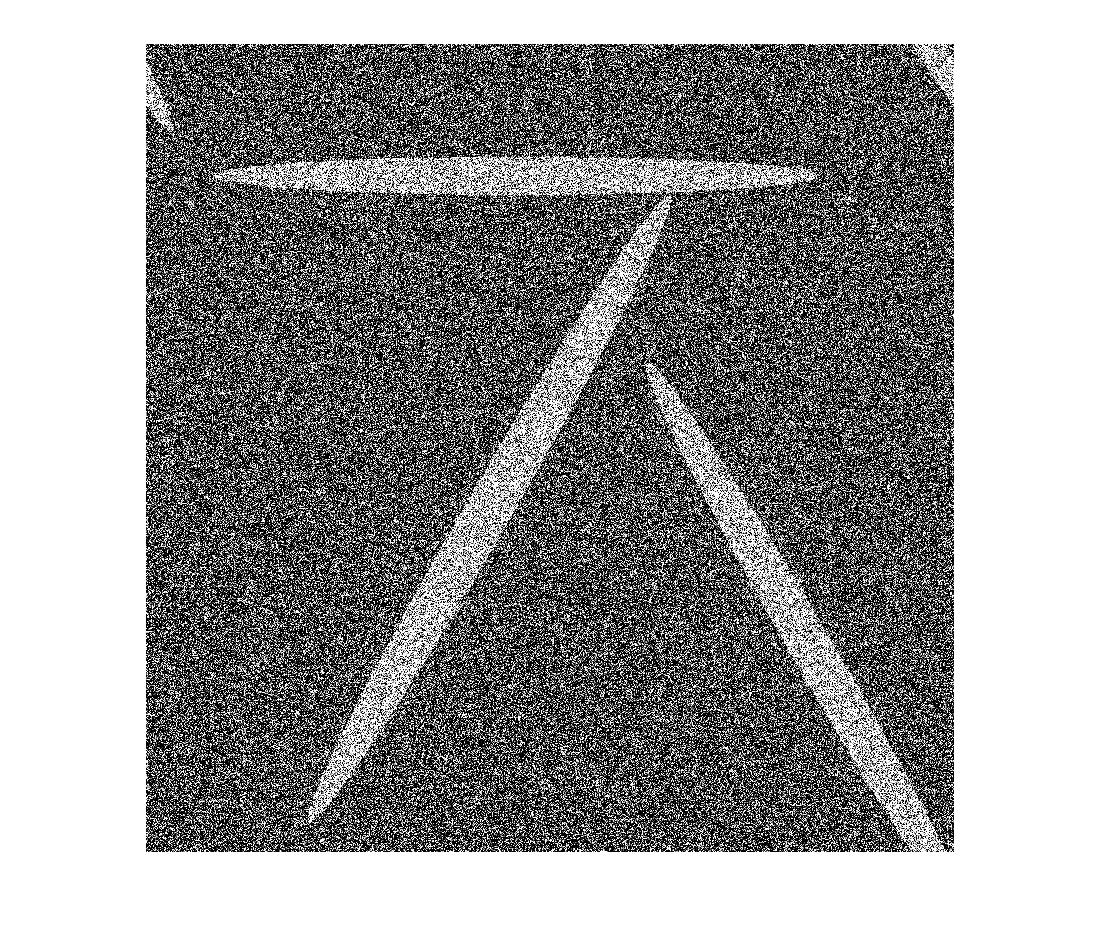
\includegraphics[scale=.11]{../../figs/ellipses_t1}
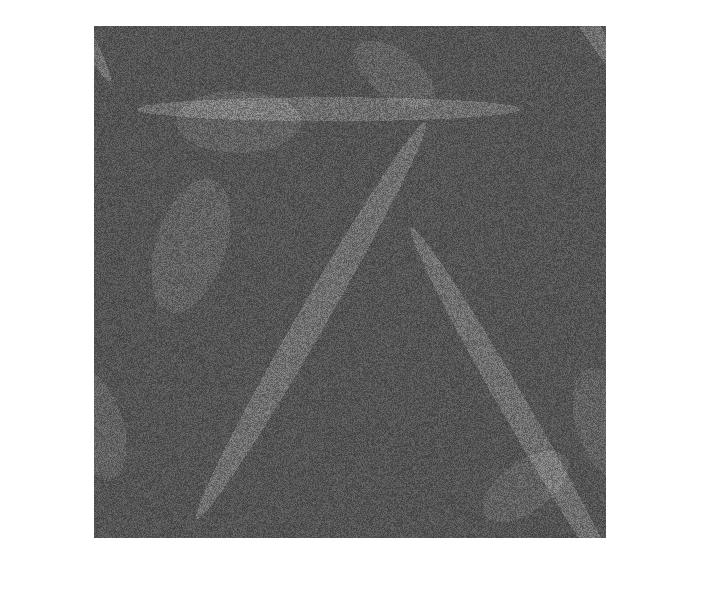
\includegraphics[scale=.11]{../../figs/ellipses_t2}
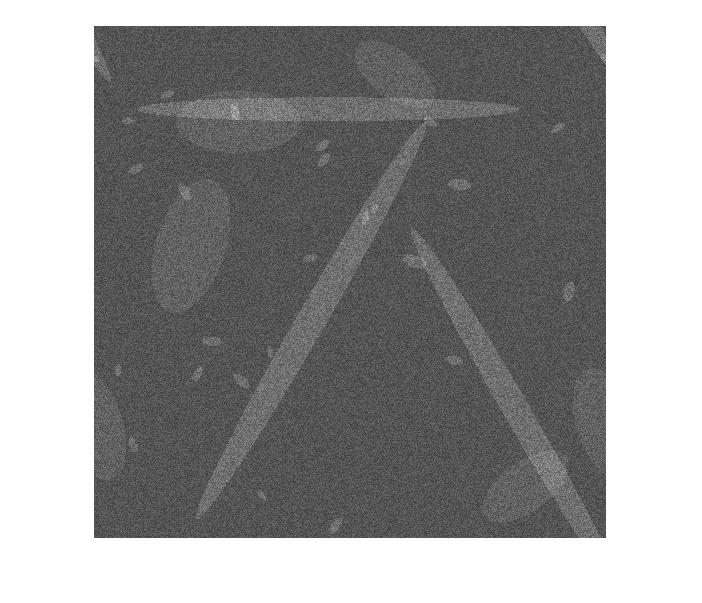
\includegraphics[scale=.11]{../../figs/ellipses_t3}
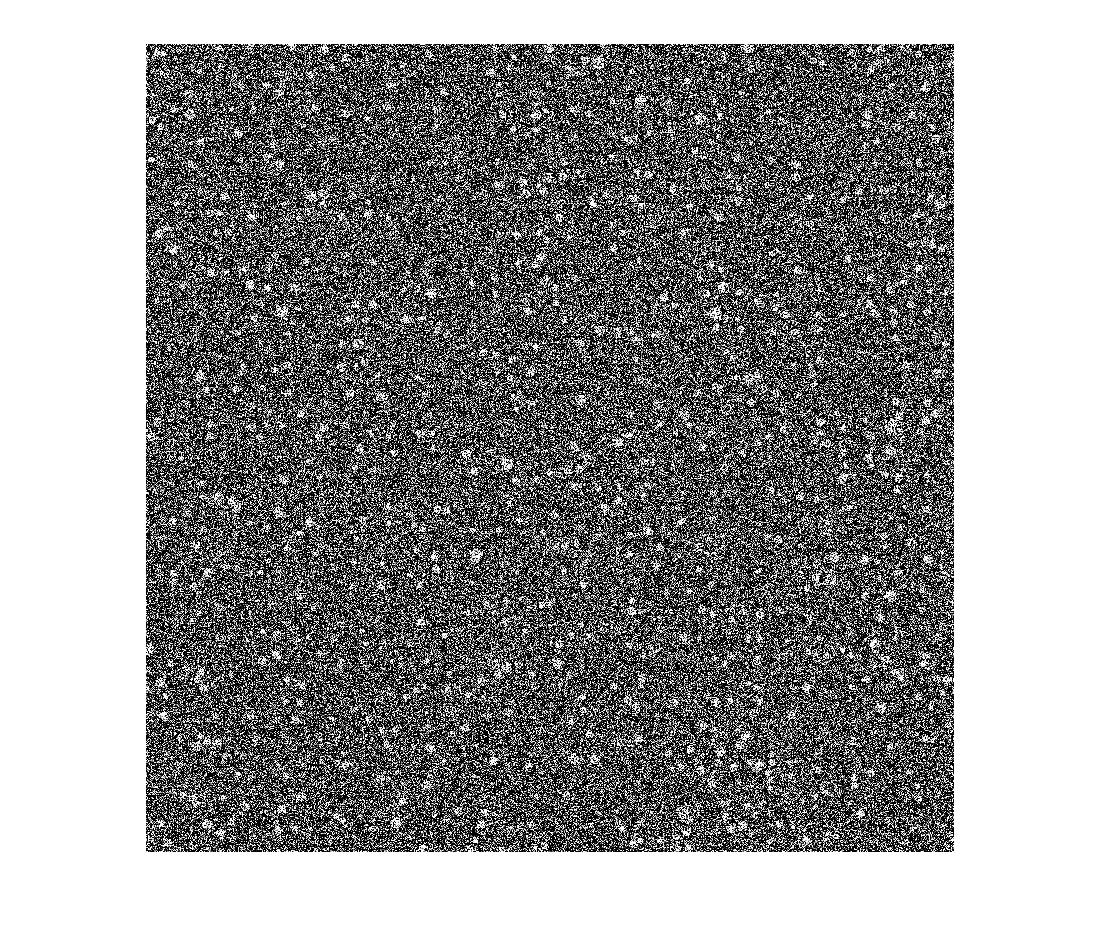
\includegraphics[scale=.11]{../../figs/ellipses_t4}
\caption{Example of the first four synthetic multi-temporal images. Features and changes come as white ellipses and dots.}
\label{F:EllipsoidChanges}
\end{figure}


\begin{figure}[htp!]
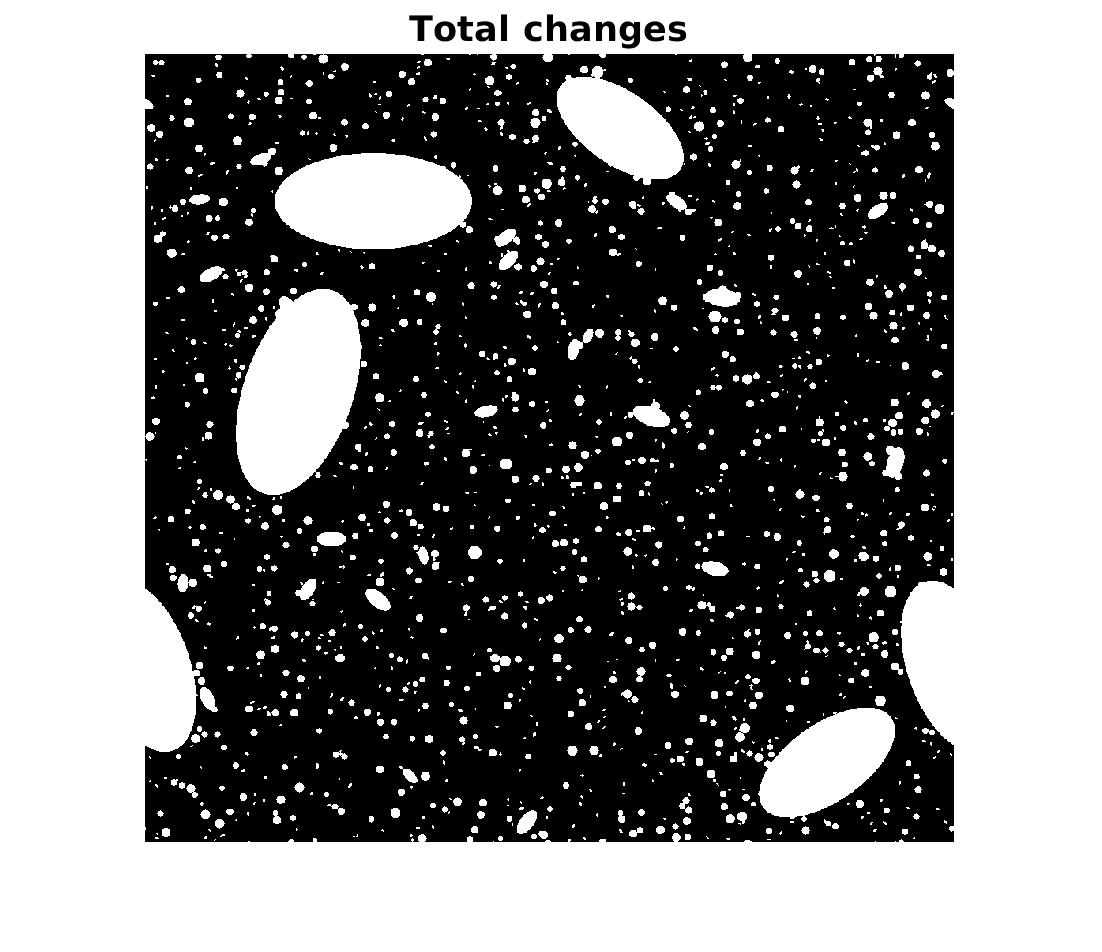
\includegraphics[scale=.1]{../../figs/total_changes}(a)
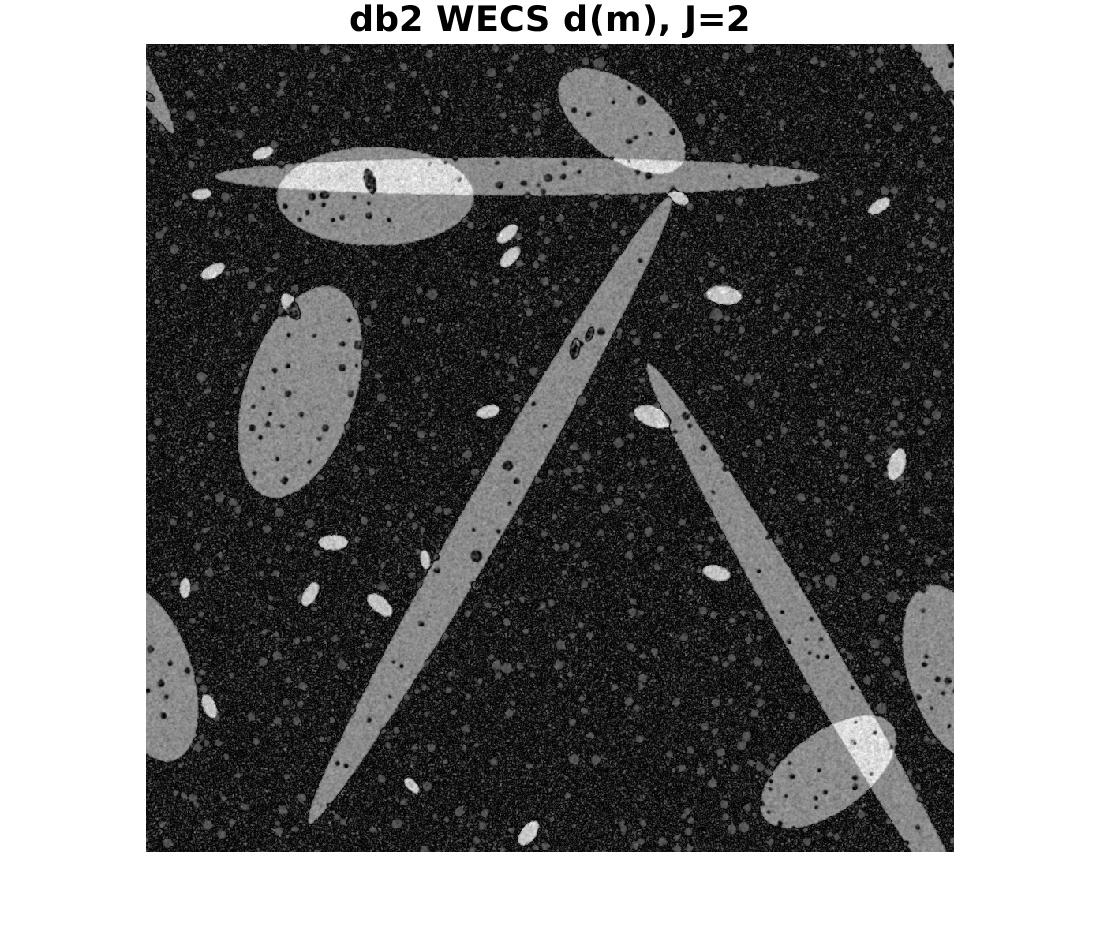
\includegraphics[scale=.1]{../../figs/corr_changes_dm}(b)
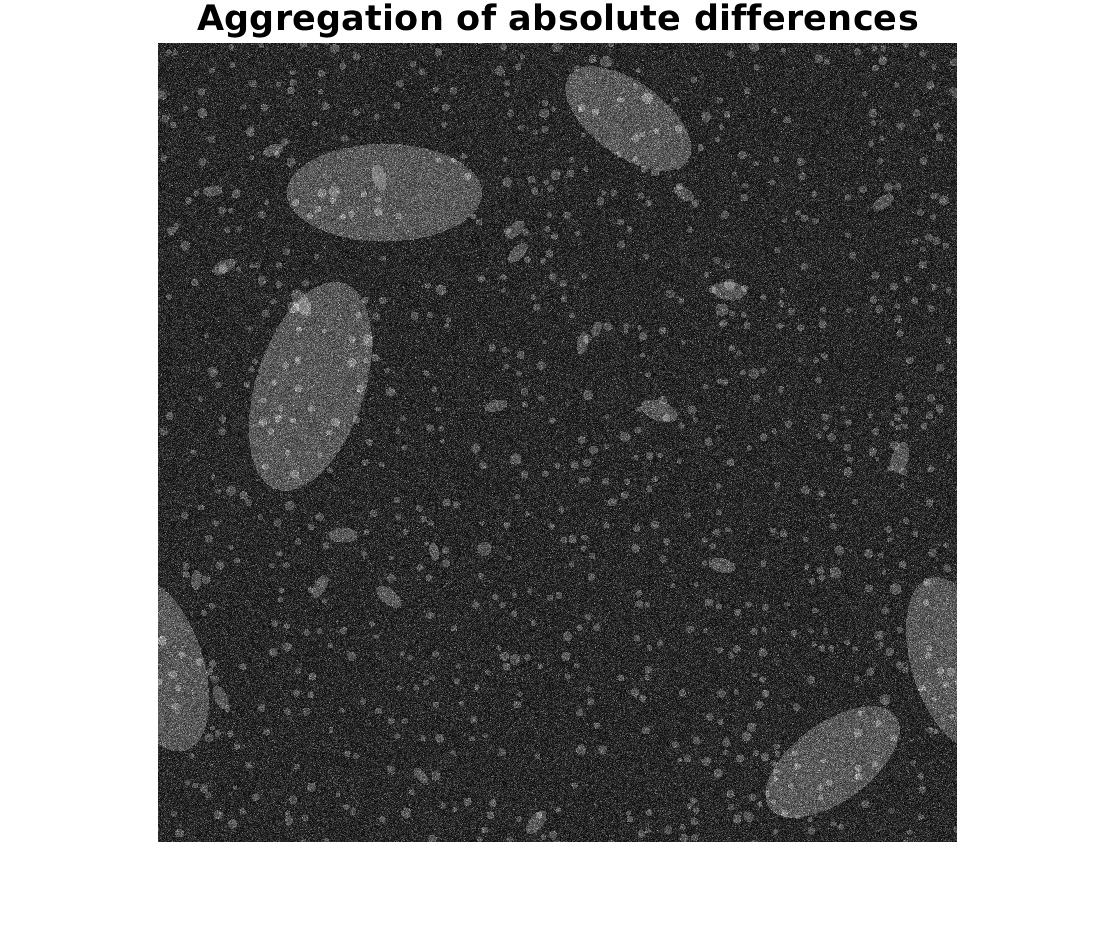
\includegraphics[scale=.1]{../../figs/corr_changes_logratios}(c)
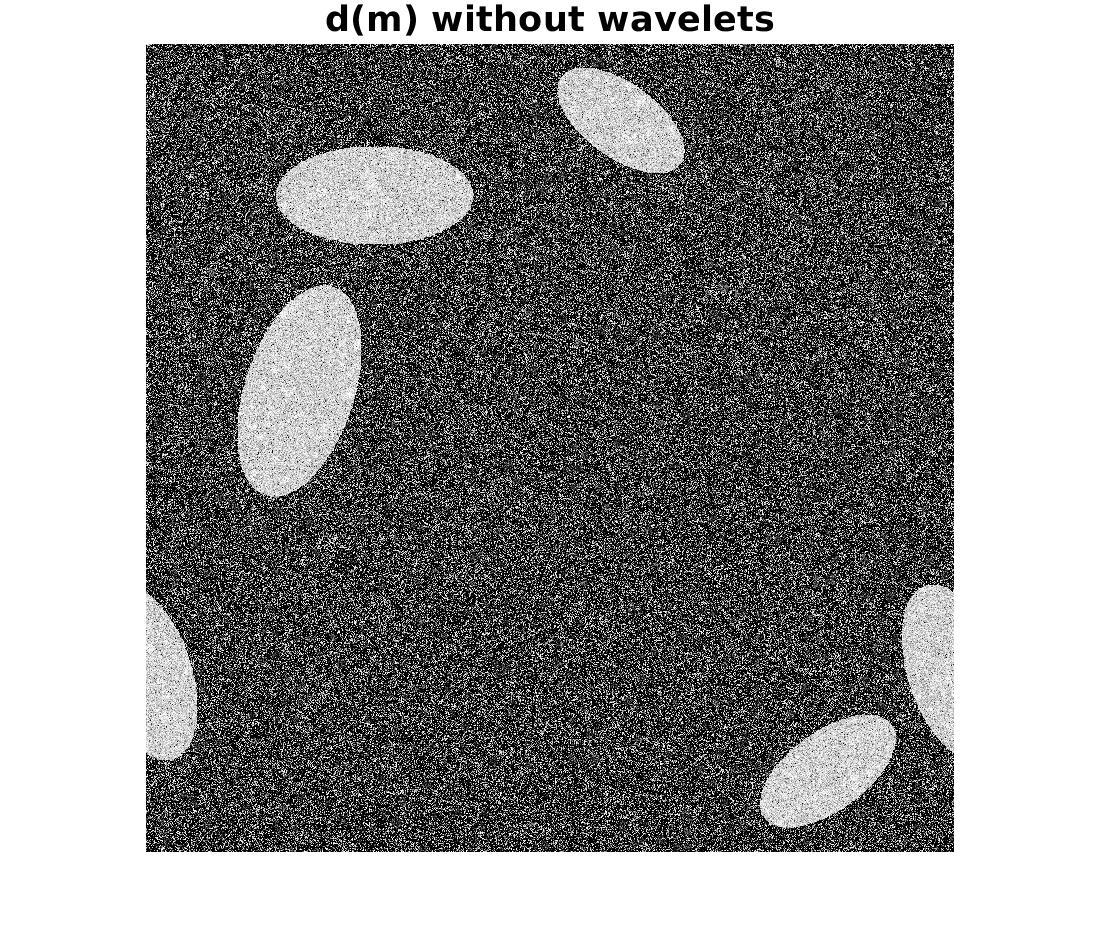
\includegraphics[scale=.1]{../../figs/corr_changes_dm_nowavelets}(d)
\caption{Synthetic images with changing ellipses. (a) Image composed by the total changes over time. (b) Proposed db2 WECS $\vd(m)$ with $J=2$; (c) Standard approach. (d) $\vd(m)$ without wavelets.}
\label{F:Changes_methods_images}
\end{figure}

Figure \ref{F:Changes_methods_images} illustrates a comparison of different approaches to detect accumulated changes. Panel (b) shows the result of WECS using Daubechies wavelet with two null moments (db2) and $J=2$. Panel (c) presents the result of using aggregated absolute differences, a standard approach where the accumulation of changes are measured by a matrix $\vS=\{\vS_{k,l}\}$ with $S_{kl} = \sum_{m=2}^n	|\mathcal{I}_{k,l}(m) - \mathcal{I}_{k,l}(m-1)|$. Finally, in Panel (d) we can see the result if $\vd(m)$ is performed purely on the spatial domain, using $\mathcal{I}(m)$ instead of $\vX(m)$ in the WECS formulation. 
%The spatio-temporal advantages of the proposed wavelet  $\vd(m)$ is clear in Figure \ref{F:Changes_methods_images}(b), which shows that a wavelet smoothing has an expressive capacity of measuring the the changes through correlations of coefficients' deviations, even for the changes corresponding to smaller ellipses.


We compute ROC curves to compare the detection performance of different methods and to verify the influence of some tuning parameters of wavelet smoothing: the resolution level $J$ and the choice of wavelet basis. Each detection method generates a matrix of change detection measures (correlations in the case of WECS). The ROC curves present the performance of change detection by applying a threshold on these measures, in the following way:
\begin{enumerate}
\item Let $R$ be the matrix of change measures. Compute the range $[r_{\min},r_{\max}]$ of the values in $R$;
\item Let $(r_{(1)},\ldots,r_{(100)})$ be equally space values between $r_{\min}$ and $r_{\max}$;
\item For each $k=1,\ldots,n$, check how many entries are there such that $R_{i,j}>r_{(k)}$ coincide with the element $(i,j)$ where a change really occurs on the image of total changes. Dividing this number by the total number of changes gives the true positive rate.
\item For each $k=1,\ldots,n$, check how many entries are there such that $R_{i,j}>r_{(k)}$  do not coincide with the element $(i,j)$ where a change really occurs. Dividing this number by the total number of entries where changes do not occur gives the false positive rate.
\item The ROC curve is the plot of true and false positive rates corresponding to each $k$.
\end{enumerate}

\begin{figure}[htp!]
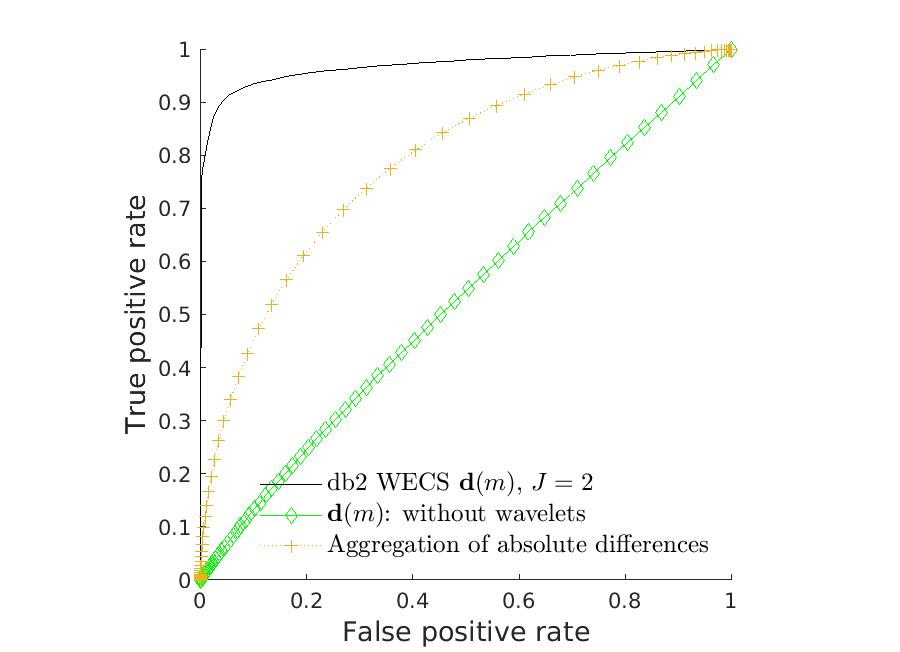
\includegraphics[scale=.13]{../../figs/methods_comparison}\hspace{-.6cm}(a) 
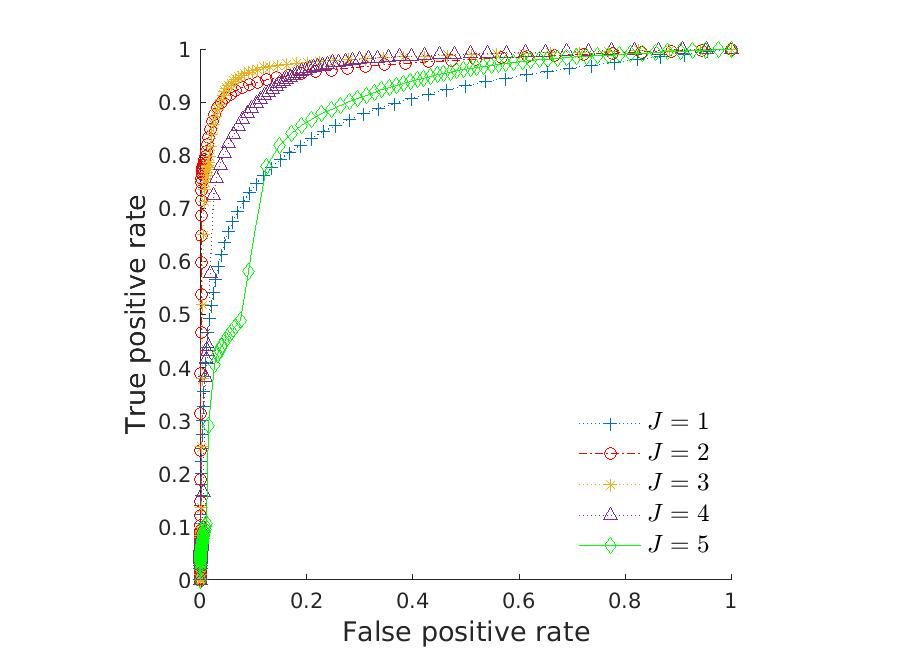
\includegraphics[scale=.13]{../../figs/levels_comparison}\hspace{-.5cm}(b)\\
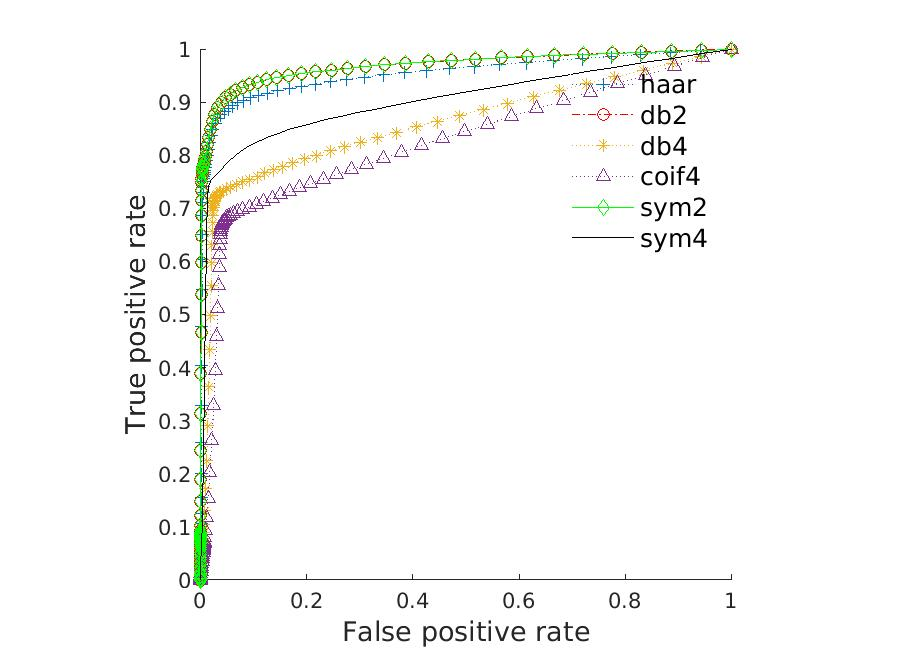
\includegraphics[scale=.13]{../../figs/families_comparison}\hspace{-.5cm}(c)
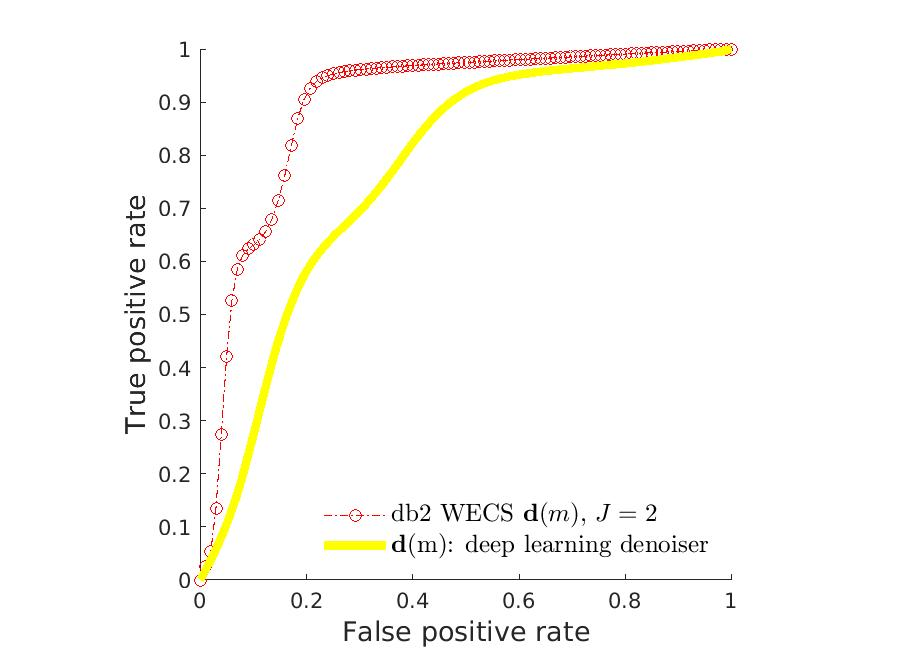
\includegraphics[scale=.13]{../../figs/dm_comparison_wavelet_deepL}\hspace{-.5cm}(d) \\
\caption{ROC curves for detection of changing ellipses in synthetic images and different methods. (a) The proposed methods in black (db2 WECS $\vd(m)$) vs two non-wavelet methods: standard log-ratio aggregation (red stars); and $\vd(m)$ (blue).
(b) db2 $\vd(m)$ with different levels.
(c) $\vd(m)$ with different wavelet bases and J=2;
(d) The proposed db2 WECS $\vd(m)$ (red circles) and $\vd(m)$ with deep-learning feature extraction and without wavelets (yellow line).}
\label{F:EllipsoidChanges_details}
\end{figure}

Figure \ref{F:EllipsoidChanges_details} presents the different ROC curves for change detection methods applied to the synthetic data as follows. The effects of wavelet bases, level of decomposition, deep-learning feature extraction are shown on the ROC curves. We employ the following wavelet bases: Haar;  Daubechies db2; Daubechies db4; Coiflets coif4; Symlets sym2 ; and Symlets sym4. Panel (c) presents the ROC curves for the proposed method under the aforementioned bases. On all instances $J=2$ is employed. Comparing the ROC curves of all options, we can notice that Daubechies db2 and Symlets sym2 are the best choices.  Panel (b) presents the ROC curves for five different levels of decomposition $J=\{1,2,3,4,5\}$ under the Daubechies db2 basis. Levels $J=2,3$ have a clear better performance, with a slight advantage to $J=2$, since it is uses less levels on the decomposition. The overall performance  of $J=2$ warrants its use for the rest of the comparisons. Panel (d) shows how the proposed method performs in comparison to a deep learning feature extraction from a residual learning network \cite{zhang2017beyond}. WECS is applied with db2 wavelets and $J=2$, whereas the other method applies WECS's idea, the only difference being that $\vX(m)$ is replaced by another smooth version of $\mathcal{I}(m)$ that employs neural-networks trained to compete with wavelet smoothing. We can see that the ROC curves for images treated with a deep-learning method has a performance worse than that obtained with WECS. 
% The WECS runs in 0.42s, while the deep-learning based $\vd(m)$ runs in 64.68s on a notebook. The configuration of the notebook is: OS - Ubuntu 18.04.5 LTS; RAM 7.7 GB; Intel\textregistered Core\texttrademark $ $i7-8565U CPU @ 1.80GHz x 8; graphics - Mesa Intel\texttrademark UHD Graphics 620 ; GNOME - 3.36.8; OS type - 64-bit. 
We finally have in Panel (a) the proposed WECS with db2 wavelets and $J=2$ compared to two other non-wavelet methods. The first involves computing $\vd(m)$ without wavelet smoothing, i.e., the squared deviations are computed using $\{\mathcal{I}(m)\}$ instead of $\{\vX(m)\}$, and the classic method of analyzing aggregated absolute differences of $\{\mathcal{I}(m)\}$. The ROC curves in Panel (a) show that the proposed WECS outperforms both the other two methods. 

%\begin{figure}[htp!]
%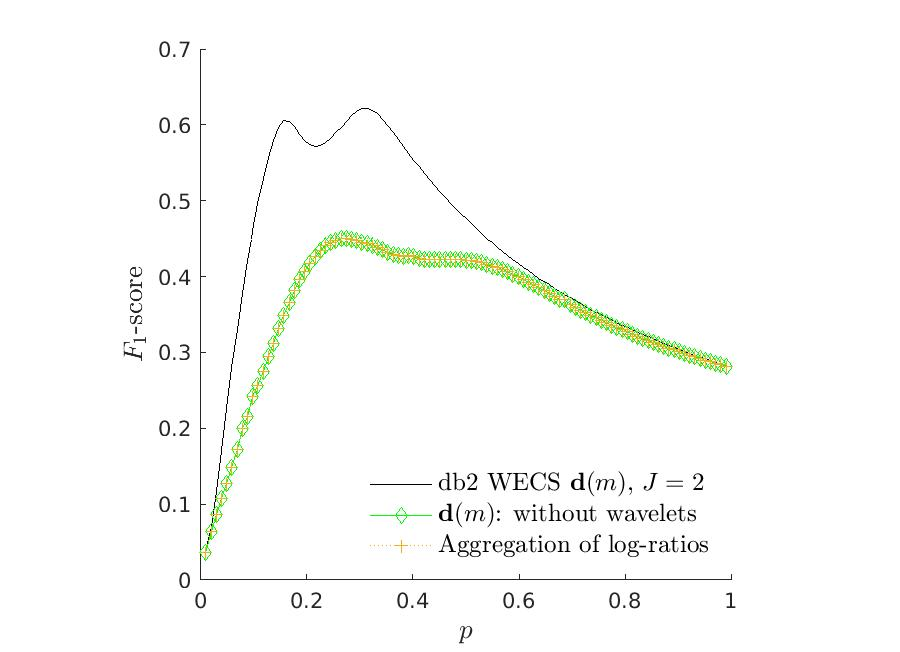
\includegraphics[scale=.14]{../../figs/methods_comparison_F1score}\hspace{-.5cm}(a) 
%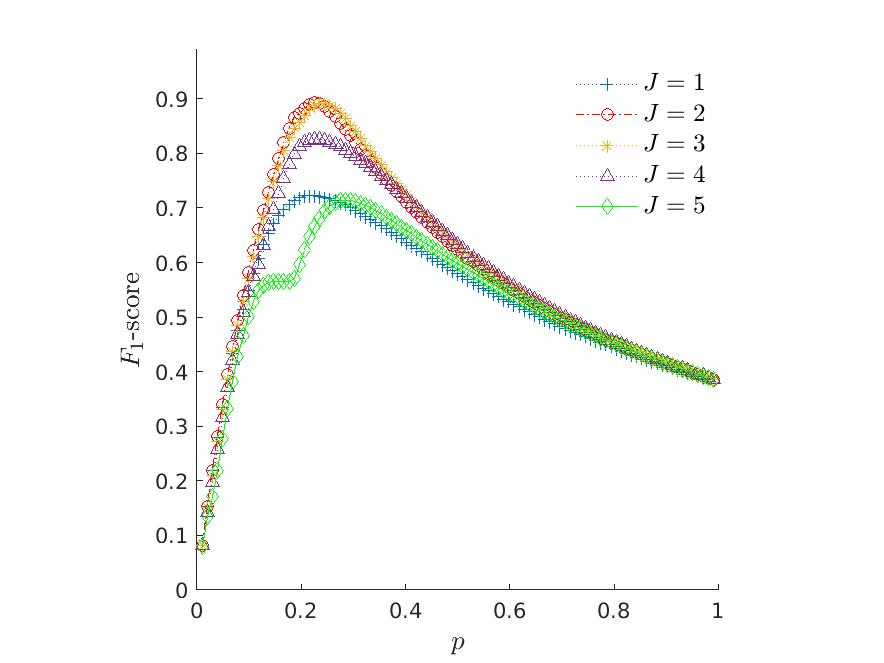
\includegraphics[scale=.14]{../../figs/levels_comparison_F1score}\hspace{-.5cm}(b)\\
%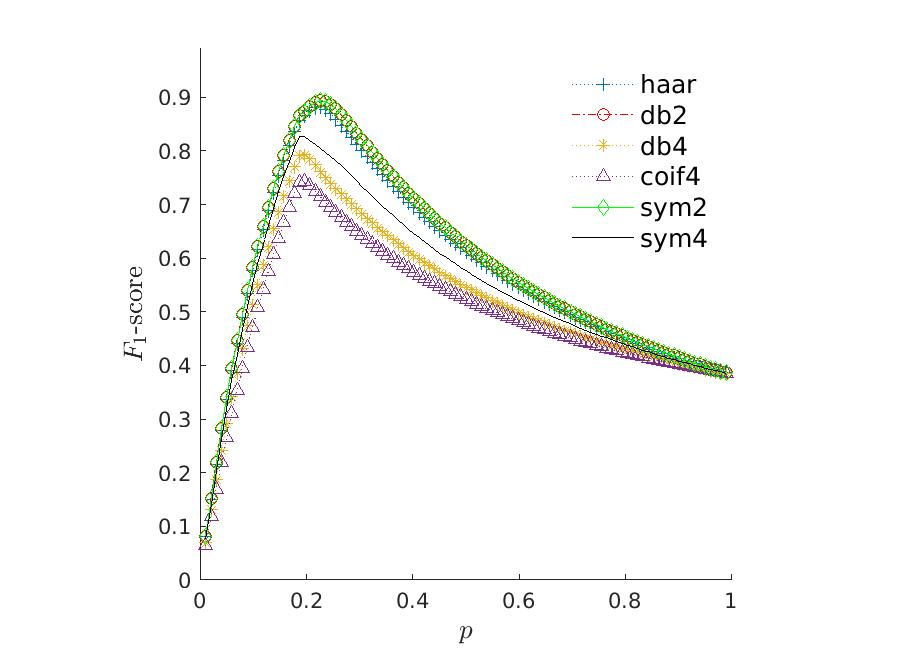
\includegraphics[scale=.14]{../../figs/families_comparison_F1score}\hspace{-.5cm}(c)
%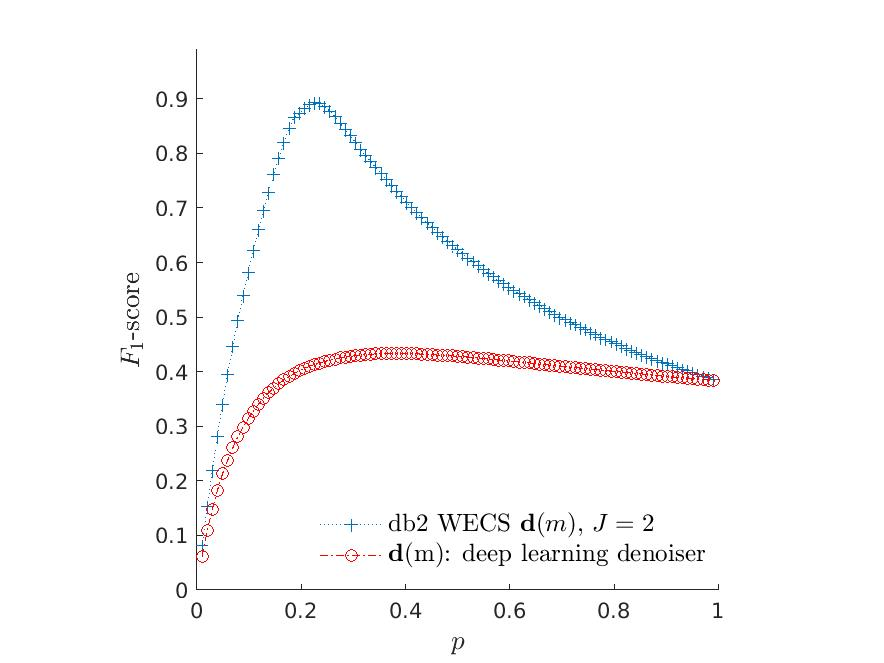
\includegraphics[scale=.14]{../../figs/dm_comparison_wavelet_deepL_F1score}\hspace{-.5cm}(d) \\
%\caption{$F_1$-scores for detection of changing ellipses in synthetic images and different methods. (a) The proposed methods in black (db2 WECS $\vd(m)$) vs two non-wavelet methods: standard log-ratio aggregation (red stars); and $\vd(m)$ (blue).
%(b) db2 $\vd(m)$ with different levels.
%(c) $\vd(m)$ with different wavelet bases and J=2;
%(d) The proposed db2 WECS $\vd(m)$ (red circles) and $\vd(m)$ with deep-learning feature extraction and without wavelets (yellow line).}
%\label{F:EllipsoidChanges_details}
%\end{figure}




%\section{Real Data Results}\label{section_realdata}
%%%%%%%%%%%%%%%%%%%%
%\subsection{Validation on synthetic data}\label{section_validation}
\subsection{Actual remote sensing application}\label{secExpActual}

We employed the proposed change detection method on a series of 84 multi-date satellite images. The images were taken on a forest region at the border of Brazil and the French Guiana (Figure~\ref{figAE}) from 26th December 2015 to 3rd December 2017. Each image has two polarizations (VV and VH) and 1538 by 1556 pixels. We perform a change detection wavelet analyses on the combined image by considering each observed entry as $\mathcal{I}_{k,l}(m) = (\mathrm{VV}_{k,l}(m)^2+\mathrm{VH}_{k,l}(m)^2)^{1/2}$, where $\mathrm{VV}$ and $\mathrm{VH}$ represent the matrices of observations from VV and VH channels, respectively. 


%-----------------------
\begin{figure}[hbt]
\centering
\includegraphics[width=0.485\textwidth]{../../qgis/maps/StudyArea.pdf}
\caption{Study area location. \textcolor{red}{(preliminar)}}\label{figAE}
\end{figure}


%-----------------------
\begin{figure}[hbt]
\centering

\mbox{
\subfigure[26th December, 2015]{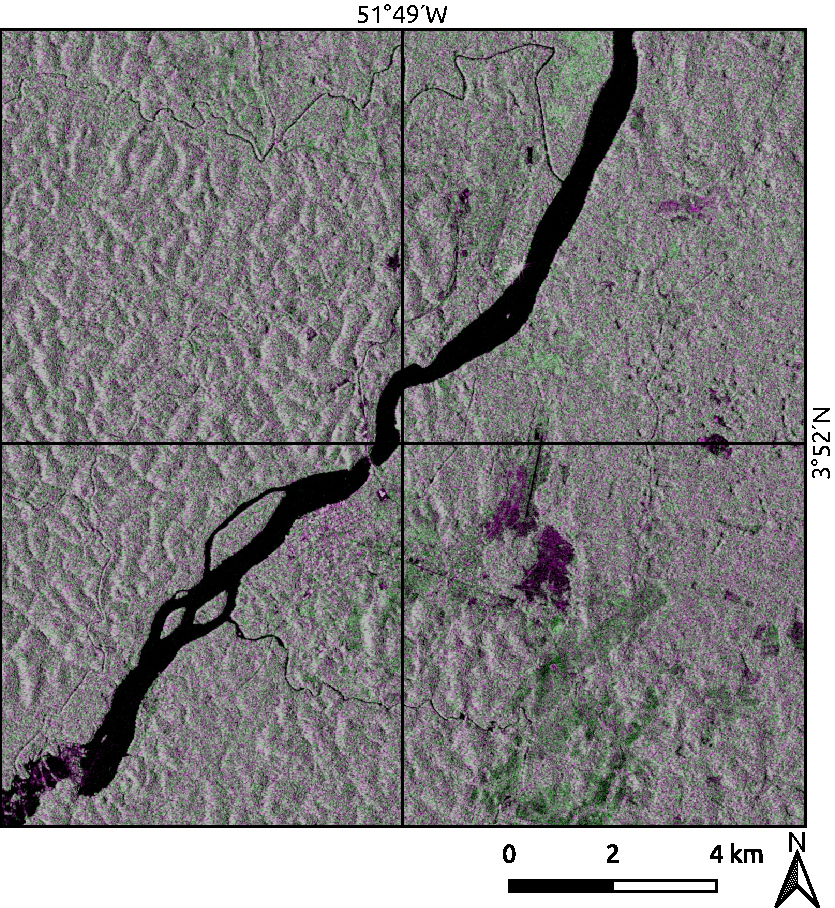
\includegraphics[width=0.23\textwidth]{../../qgis/maps/Sentinel_2015.pdf}\label{figImgSentinel2015}} 
\subfigure[3rd December, 2017]{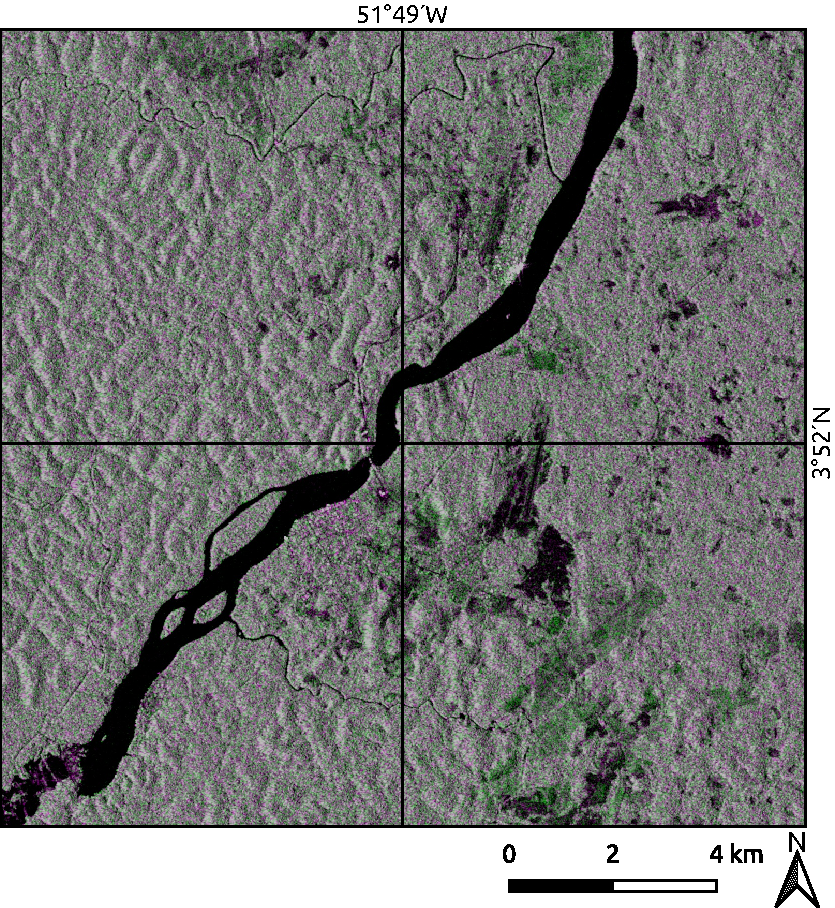
\includegraphics[width=0.23\textwidth]{../../qgis/maps/Sentinel_2017.pdf}\label{figImgSentinel2017}}
}

\subfigure[Ground truth change/non-change samples]{
\includegraphics[width=0.23\textwidth]{../../figs/coming-soon.png}\label{figImgSentinelROIs}}

\caption{\textcolor{red}{Inserir caption...}}\label{figImageRef}
\end{figure}



A multi-resolution analysis (MRA) based on a Symlet basis with filter of length 16 (symlet 8) is built. In order to have dimensions as power of 2, the matrices $\mathcal{I}_{k,l}$ were extended to a $2048\times2048$ matrix with $\mathcal{I}_{k,l}$ at the center and the remaining parts being completed with mirrored values at the borders. The wavelet transform at resolution level $J=2$ was applied to these matrices. Then, we are able to compute the squared mean differences vector $\vd$ and the matrix of absolute correlations $\vR$. 

The time change measures computed with $\vd$ are shown in Figure \ref{F:forest_wecs}a. The orange line in Figure \ref{F:forest_wecs}a represents the median absolute deviation of $\vd$, which allow us to notice times that differ expressively from the others. We can notice that times $m=25,27,30$ are highlighted as having expressive changes. The images  corresponding to these times can be seen in Figure \ref{F:forest_change_times}.

The changes in space can be analyzed using the image obtained with $\vR$, which is displayed in Figure \ref{F:forest_wecs}b. Taking the $[n/\log n]$ ($n=1538\times1556$) largest absolute correlations as those corresponding to possible change points, we obtain a matrix of zeros and ones that is presented in Figure \ref{F:forest_wecs}c. The white regions in Figure \ref{F:forest_wecs}c (entries with value one) represent the change points, which seem to concentrate mainly on three regions: at the center, to the right of the river; at the top, on the left border of the river; and at the top left. Computing aggregated absolute differences to measure changes in space, we obtain Figure \ref{F:forest_wecs}d. The first two regions captured using WECS are also detected in Figure \ref{F:forest_wecs}d, but the former offers higher contrasts to these change regions. The comparison between the performance of these two methods can also be checked in Figure \ref{F:forest_roc_wecs_agg}, where a ROC curve is computed to check the correct detection of changing and not-changing regions. These change/nonchange regions were determined using [XXXXX]. We can notice that WECS reaches high correct detection earlier than the method that uses aggregation of differences, but both methods do not have good performances concerning the nonchange regions.

\begin{figure}[htp!]
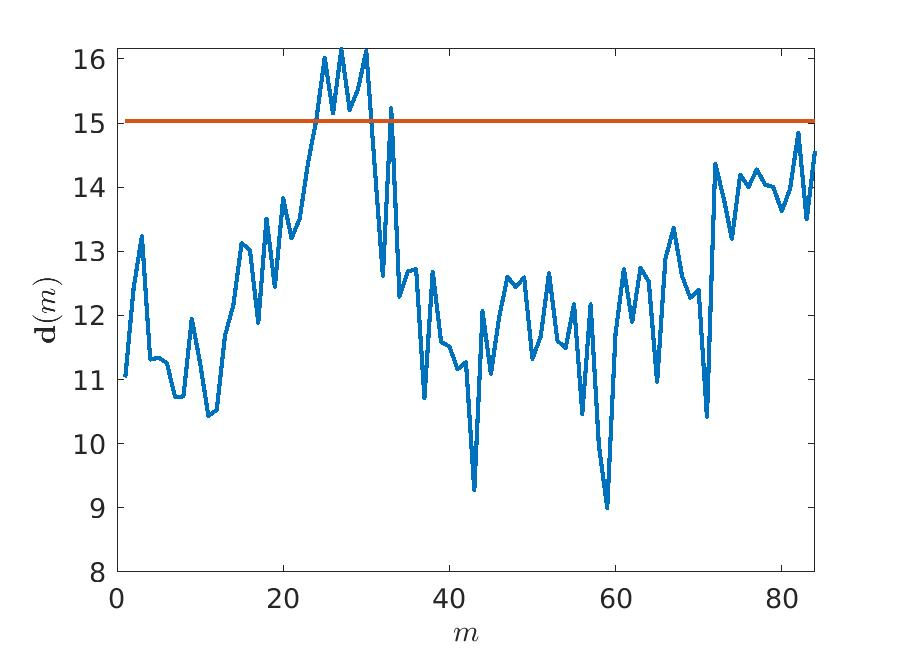
\includegraphics[scale=.13]{../../figs/forest_vSumDifCoefSq}\hspace{-.5cm}(a) 
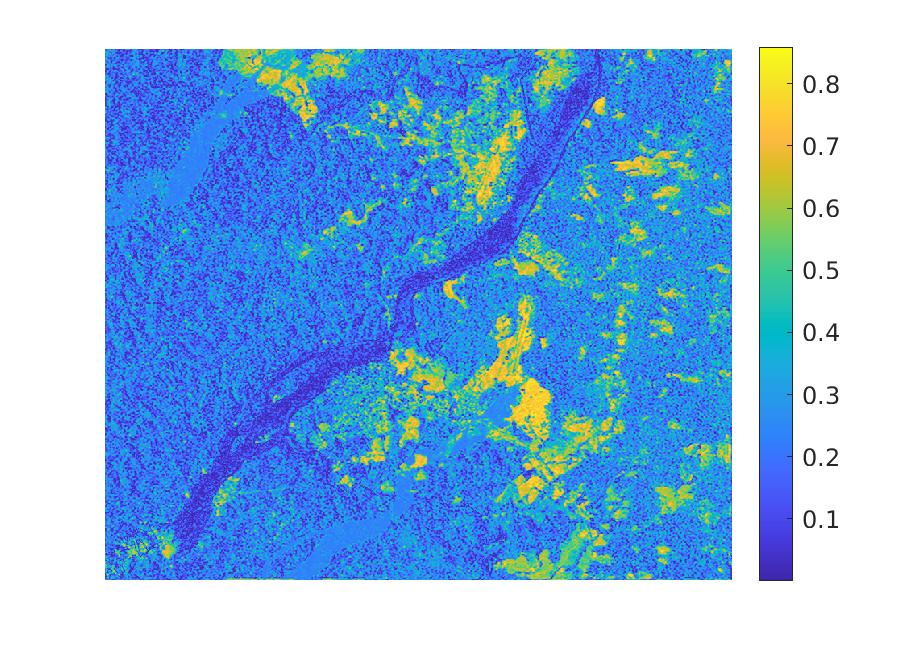
\includegraphics[scale=.14]{../../figs/forest_wecs_abscorr}\hspace{-.5cm}(b)\\
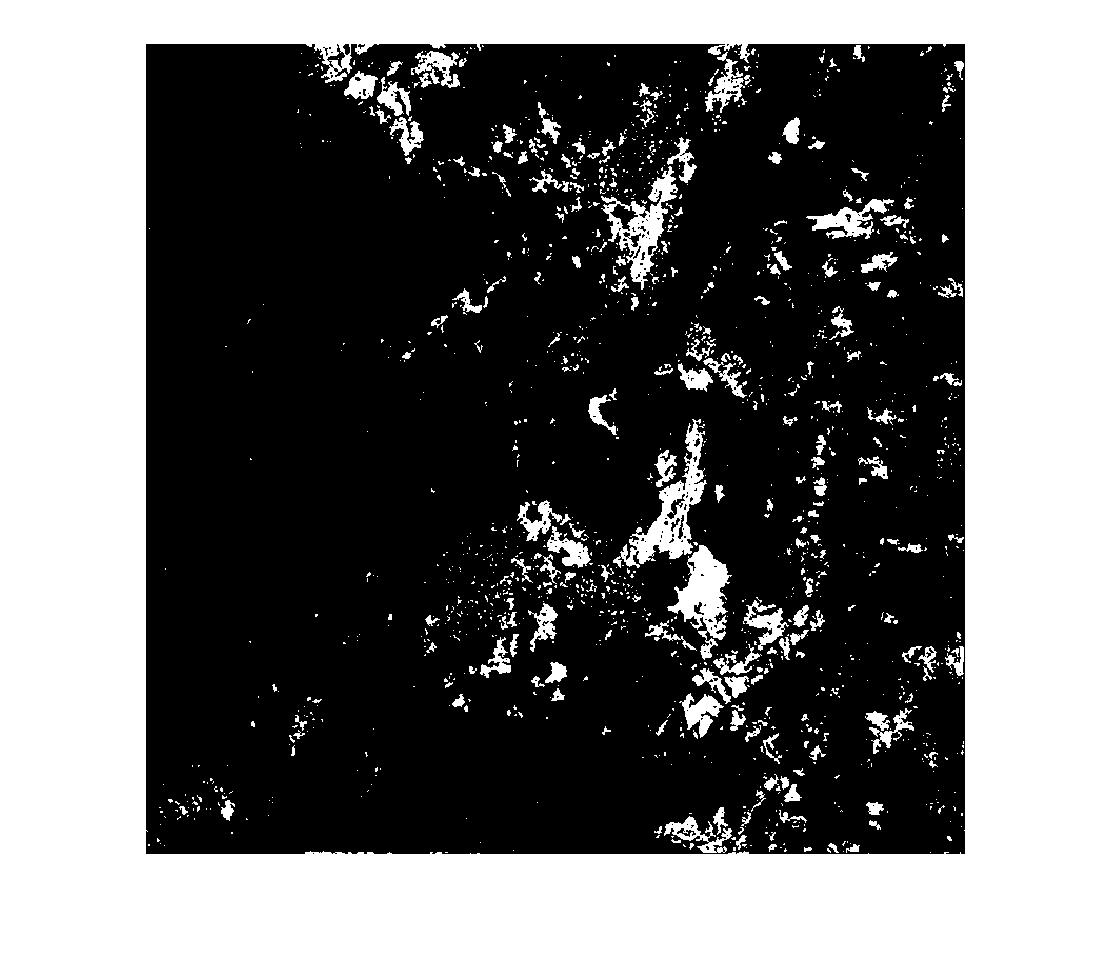
\includegraphics[scale=.10]{../../figs/forest_wecs_change_space}\hspace{-.5cm}(c) 
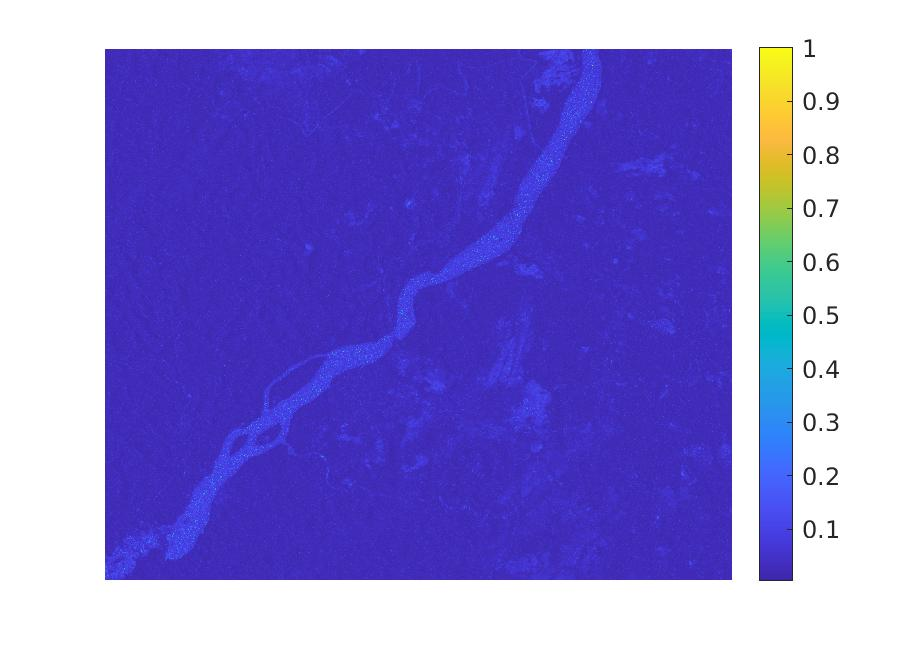
\includegraphics[scale=.14]{../../figs/forest_aggreg_ratios}\hspace{-.5cm}(d)\\ 
\caption{Analysis of change points in time and space of the forest data. (a) Plot of $\vd(m)$, $m=1,\ldots,85$ with orange horizontal line indicating two times its median absolute deviation. (b) Matrix of absolute correlations obtained with WECS. (c) Change regions detected by highlighting the $[n/\log n]$ largest correlations. (d) Change measured with aggregation of absolute differences.}
\label{F:forest_wecs}
\end{figure}


\begin{figure}[htp!]
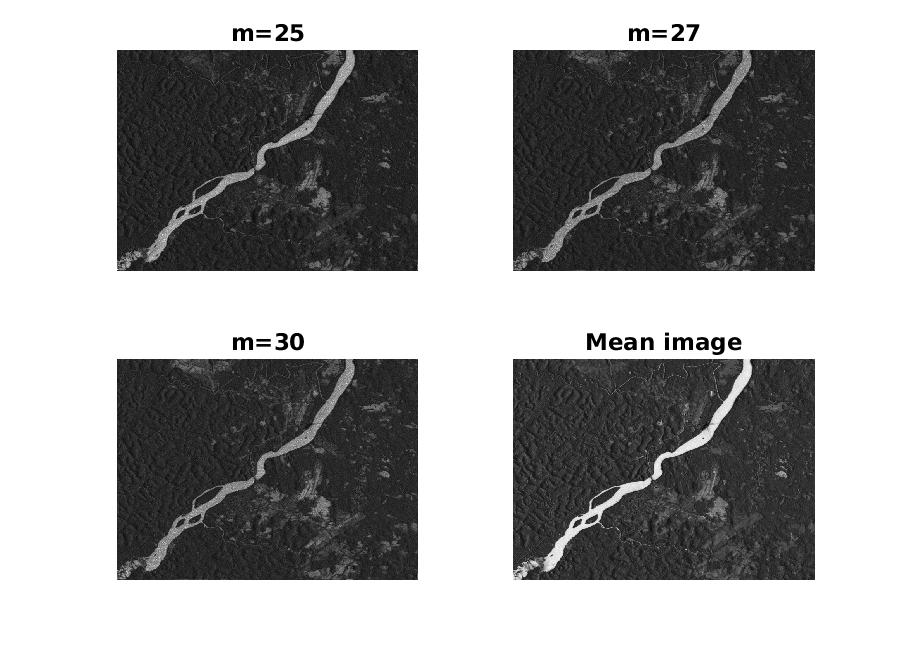
\includegraphics[scale=.3]{../../figs/forest_changes_time} 
\caption{Images whose time $m$ correspond to points of $\vd(m)$ above two times its median absolute deviation in Figure \ref{F:forest_wecs}a.}
\label{F:forest_change_times}
\end{figure}

\begin{figure}[htp!]
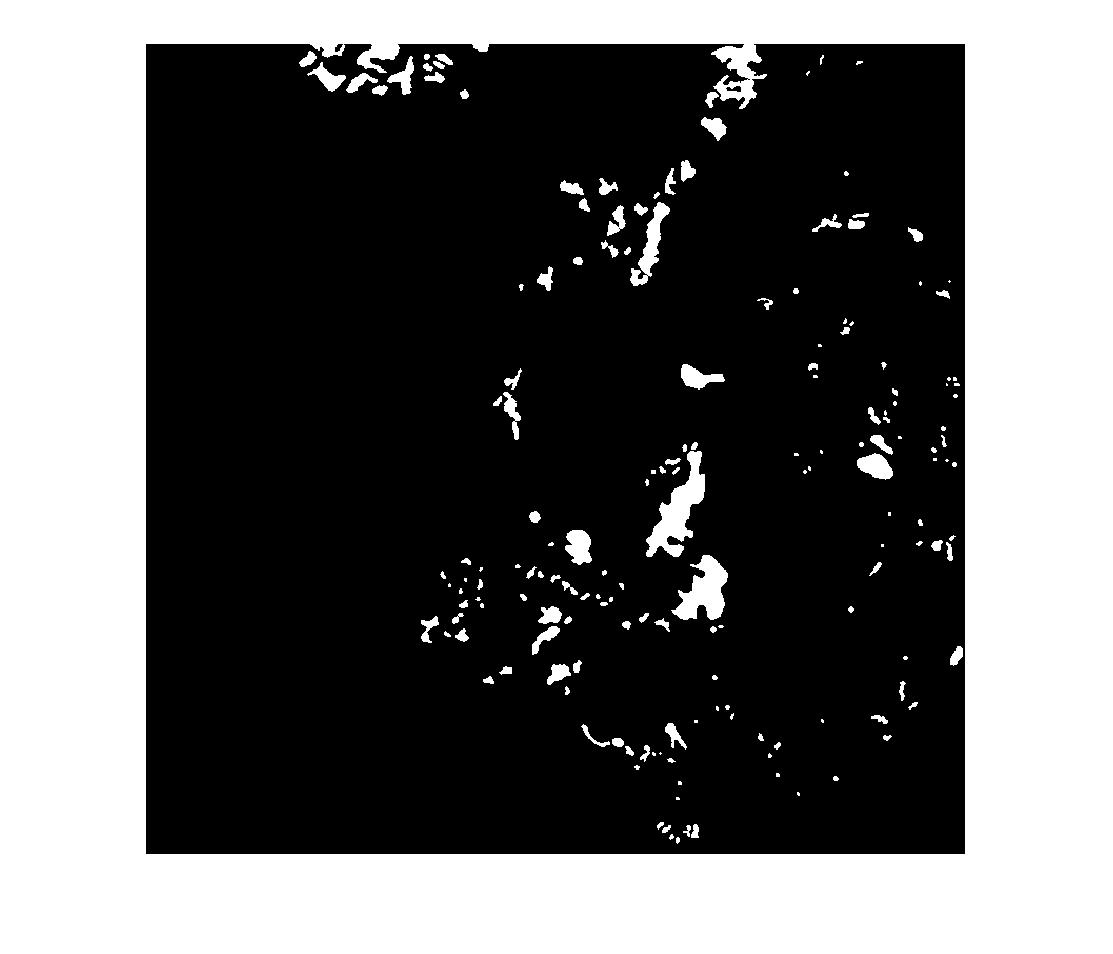
\includegraphics[scale=.11]{../../figs/forest_change}\hspace{-.5cm}(a)
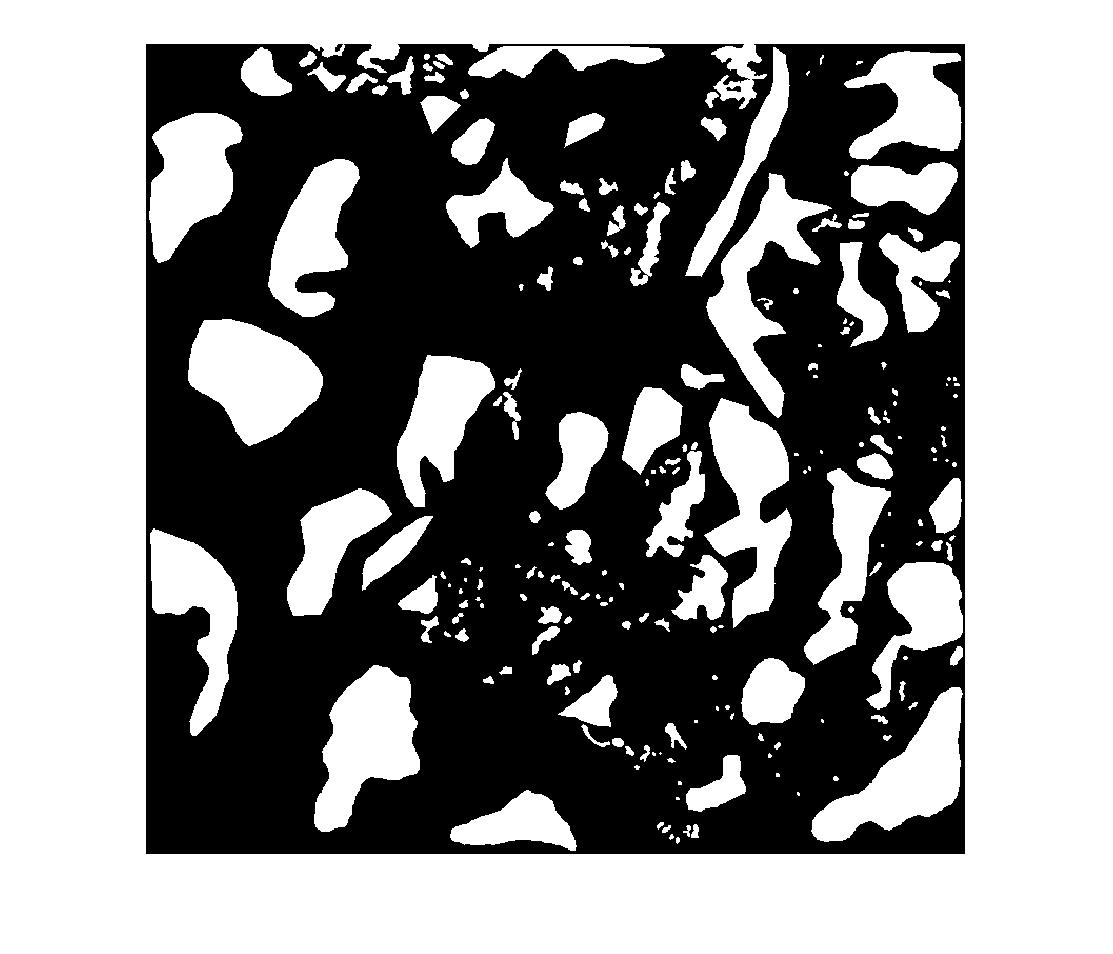
\includegraphics[scale=.11]{../../figs/forest_nonchange}\hspace{-.5cm}(b)\\
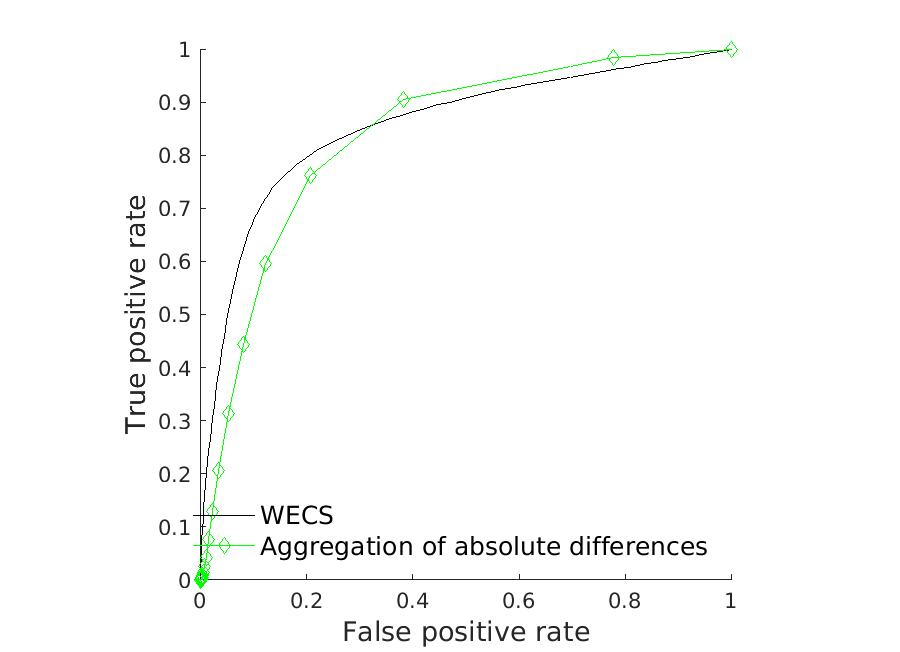
\includegraphics[scale=.13]{../../figs/forest_roc_change}\hspace{-.5cm}(c) 
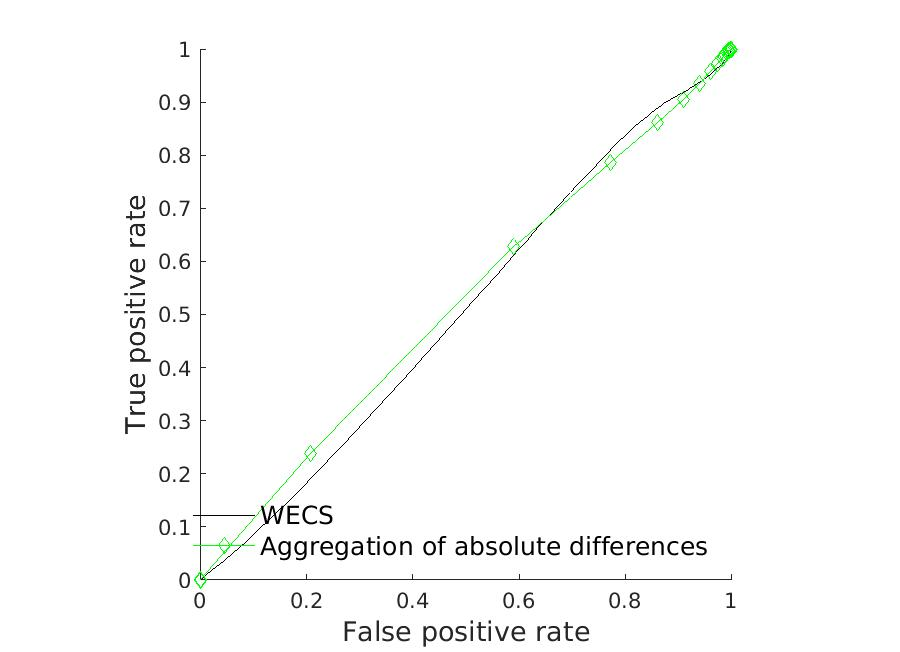
\includegraphics[scale=.14]{../../figs/forest_roc_nonchange}\hspace{-.5cm}(d)
\caption{Analysis of change points in time and space of the forest data. (a) Regions (in white) where changes should be detected. (a) Regions (in white) where changes are not expected to be detected. (c) ROC curve for detection of changing regions. (d) ROC curves for detection of nonchange regions.}
\label{F:forest_roc_wecs_agg}
\end{figure}


\section{Discussion}\label{section_discussion}

We present a novel way of detecting changes in multi-temporal satellite images, WECS. The procedure is based on wavelet energies from both the estimated individual coefficients as well as the whole mean image. It makes use of correlation screening for ultra-high dimensional data. The proposed method's performance is shown using both synthetic and real data. The proposed method is useful to detect spatio-temporal change points, which is illustrated on data analyses. The method is employed to analyze a time series of 84 images of a forest.




% if have a single appendix:
%\appendix[Proof of the Zonklar Equations]
% or
%\appendix  % for no appendix heading
% do not use \section anymore after \appendix, only \section*
% is possibly needed

% use appendices with more than one appendix
% then use \section to start each appendix
% you must declare a \section before using any
% \subsection or using \label (\appendices by itself
% starts a section numbered zero.)
%

%
%\appendices
%\section{Proof of the First Zonklar Equation}
%Appendix one text goes here.

% you can choose not to have a title for an appendix
% if you want by leaving the argument blank
%\section{}
%Appendix two text goes here.


% use section* for acknowledgment
%\section*{Acknowledgment}



% Can use something like this to put references on a page
% by themselves when using endfloat and the captionsoff option.
\ifCLASSOPTIONcaptionsoff
  \newpage
\fi



% trigger a \newpage just before the given reference
% number - used to balance the columns on the last page
% adjust value as needed - may need to be readjusted if
% the document is modified later
%\IEEEtriggeratref{8}
% The "triggered" command can be changed if desired:
%\IEEEtriggercmd{\enlargethispage{-5in}}

% references section

% can use a bibliography generated by BibTeX as a .bbl file
% BibTeX documentation can be easily obtained at:
% http://mirror.ctan.org/biblio/bibtex/contrib/doc/
% The IEEEtran BibTeX style support page is at:
% http://www.michaelshell.org/tex/ieeetran/bibtex/
\bibliographystyle{IEEEtran}
% argument is your BibTeX string definitions and bibliography database(s)
\bibliography{bibfile}
%
%% <OR> manually copy in the resultant .bbl file
%% set second argument of \begin to the number of references
%% (used to reserve space for the reference number labels box)
%\begin{thebibliography}{1}
%
%\bibitem{IEEEhowto:kopka}
%H.~Kopka and P.~W. Daly, \emph{A Guide to \LaTeX}, 3rd~ed.\hskip 1em plus
%  0.5em minus 0.4em\relax Harlow, England: Addison-Wesley, 1999.
%
%\end{thebibliography}

% biography section
% 
% If you have an EPS/PDF photo (graphicx package needed) extra braces are
% needed around the contents of the optional argument to biography to prevent
% the LaTeX parser from getting confused when it sees the complicated
% \includegraphics command within an optional argument. (You could create
% your own custom macro containing the \includegraphics command to make things
% simpler here.)
%\begin{IEEEbiography}[{\includegraphics[width=1in,height=1.25in,clip,keepaspectratio]{mshell}}]{Michael Shell}
% or if you just want to reserve a space for a photo:


%\begin{IEEEbiography}
%[{\includegraphics[width=1in,height=1.25in,clip,keepaspectratio]{../Photo/rodney}}]{Rodney Fonseca}
%was born in Brazil, in 1993. He received the Master’s
%degrees in Statistics from the Federal University of Pernambuco,
%Recife, Brazil, in 2017, and the Ph.D. degree in Statistics, from Campinas State University, Campinas, Brazil, in 2021.
%His research interests include nonparametric statistics, time series, graph signal processing and regression models.
%\end{IEEEbiography}
%\vfill
%
%\begin{IEEEbiography}[{\includegraphics[width=1in,height=1.25in,clip,keepaspectratio]{../Photo/aluisio}}]{Alu\'{i}sio~Pinheiro}
%was born in Brazil, in 1967. He received the Master’s degree in Statistics from Campinas State University, Campinas, Brazil, in 1992, and the Ph.D. degree in Statistics from University of North Carolina, Chapel Hill, US, in 1997.
%He is currently Professor at Campinas State University. His research interests concern U-statistics, wavelets, nonparametric statistics and time series.
%Dr. Pinheiro was the 2012 Pranab Kumar Sen Distinguished Visiting Professor of Biostatistics, UNC-Chapel Hill. He has been the Brazilian Statistics Association General Secretary (2010-2012) and Treasurer (2018-2020).
%\end{IEEEbiography}
%
%
%\begin{IEEEbiography}[{\includegraphics[width=1in,height=1.25in,clip,keepaspectratio]{../Photo/abdou}}]{Abdourrahmane Mahamane Atto}
%was born in Niger, in 1974. He received the Master’s
%degrees in applied mathematics and pure mathematics from the University of Abomey-Calavi,
%Cotonou, Benin, 2001 and 2002, respectively, the
%Master’s degree of advanced studies in electrical engineering from the École Polytechnique d’Abomey-Calavi, Cotonou, in 2002, and the Ph.D. degree
%in applied mathematics, codelivered by TELECOM
%Bretagne, Brest, France, and the University of
%Rennes I, Rennes, France, in 2008.
%He worked with École Polytechnique d’Abomey-Calavi, from 2002 to 2003,
%Ecole des Mines, de l’Industrie et de la Géologie, Niamey, Niger, from 2003
%to 2004, TELECOM Bretagne, from 2008 to 2009, and Institut Polytechnique
%de Bordeaux, Talence, France, from 2009 to 2011. Since September 2011, he
%has been an Associate Professor at the University of Savoie, Polytech Annecy-Chambéry, Annecy, France. His research interests concern mathematical methods and models for signal, image, and information processing.
%\end{IEEEbiography}
%\vfill

% You can push biographies down or up by placing
% a \vfill before or after them. The appropriate
% use of \vfill depends on what kind of text is
% on the last page and whether or not the columns
% are being equalized.

%\vfill

% Can be used to pull up biographies so that the bottom of the last one
% is flush with the other column.
%\enlargethispage{-5in}



% that's all folks
\end{document}


